%%%%%%%%%%%%%%%%%%%%%%%%%%%%%%%% COMMENT THIS TO COMPILE main.tex %%%%%%%%%%%%%%%%%%%%%%%%%%%%%%%%
%\documentclass[a4paper,12pt]{report}
\usepackage[english]{babel}
\usepackage[left=2cm,right=2cm,top=2cm,bottom=2cm]{geometry}
%\usepackage{mathtools}
\usepackage{amsthm}     % for definitions and theorems
\usepackage[many]{tcolorbox}    % boxes around definitions and theorems
%\usepackage{amsmath}
%\usepackage{nccmath}
\usepackage{amssymb}    % \ltimes
\usepackage{etoolbox}   % for start of Chapter
%\usepackage{amsfonts}
\usepackage{physics}    % for all Physics related
\usepackage{dsfont}     % for the identity matrix symbol \1
%\usepackage{mathrsfs}

\usepackage{titling}
\usepackage{indentfirst}

\usepackage{bm}
\usepackage[dvipsnames]{xcolor}
\usepackage{cancel}

\usepackage{xurl}
\usepackage[colorlinks=true]{hyperref}

\usepackage{float}
\usepackage{graphicx}
\usepackage{subcaption}
%\usepackage{tikz}

\usepackage{ctable}     % tabelas
\renewcommand{\P}{\phantom{+}}  % empty space to indent things
\usepackage{multirow}
\usepackage{tabulary}

%%%%%%%%%%%%%%%%%%%%%%%%%%%%%%%%%%%%%%%%%%%%%%%%%%%

\newcommand{\eps}{\epsilon}
\newcommand{\vphi}{\varphi}
\newcommand{\cte}{\text{cte}}

\newcommand{\N}{{\mathbb{N}}}
\newcommand{\Z}{{\mathbb{Z}}}
%\newcommand{\Q}{{\mathbb{Q}}}
\newcommand{\C}{{\mathbb{C}}}
\renewcommand{\S}{{\hat{S}}}
%\renewcommand{\H}{\s{H}}

\renewcommand{\a}{{\vb{a}}}
\renewcommand{\b}{{\vb{b}}}
\renewcommand{\d}{{\dagger}}
\newcommand{\up}{{\uparrow}}
\newcommand{\down}{{\downarrow}}
\newcommand{\hc}{{\text{h.c.}}}

\newcommand{\ihat}{\bm{\hat{\imath}}}
\newcommand{\jhat}{\bm{\hat{\jmath}}}
\newcommand{\khat}{\bm{\hat{k}}}

\newcommand{\0}{{\vb{0}}}
\newcommand{\1}{\mathds{1}}
\newcommand{\E}{{\vb{E}}}
\newcommand{\B}{{\vb{B}}}
\renewcommand{\u}{{\vb{u}}}
\renewcommand{\v}{{\vb{v}}}
\renewcommand{\r}{{\vb{r}}}
\newcommand{\R}{{\vb{R}}}
\newcommand{\Q}{{\vb{Q}}}
\newcommand{\G}{{\vb{G}}}
\newcommand{\g}{{\vb{g}}}
\renewcommand{\k}{{\vb{k}}}
\newcommand{\K}{{\vb{K}}}
\newcommand{\p}{{\vb{p}}}
\newcommand{\q}{{\vb{q}}}
\newcommand{\F}{{\vb{F}}}
\renewcommand{\t}{{\vb{t}}}
\newcommand{\vtau}{{\bm{\tau}}}
\newcommand{\vdelta}{{\bm{\delta}}}

% COLORED SYMMETRY ELEMENTS
\newcommand{\Ct}{{\textcolor{Cyan}{C_3}}}
\newcommand{\Ctn}[1]{{\textcolor{Cyan}{C_3^{\textcolor{black}{#1}}}}}
\newcommand{\Cs}{{\textcolor{ForestGreen}{C_6}}}
\newcommand{\Csn}[1]{{\textcolor{ForestGreen}{C_6^{\textcolor{black}{#1}}}}}
\newcommand{\sd}{{\textcolor{RoyalBlue}{\sigma_d}}}
\newcommand{\sdn}[1]{{\textcolor{RoyalBlue}{\sigma_d^{\textcolor{black}{#1}}}}}
\newcommand{\sdp}{{\textcolor{RoyalBlue}{\sigma_d'}}}
\newcommand{\sdpp}{{\textcolor{RoyalBlue}{\sigma_d''}}}
\newcommand{\sv}{{\textcolor{Orange}{\sigma_v}}}
\newcommand{\svn}[1]{{\textcolor{Orange}{\sigma_v^{\textcolor{black}{#1}}}}}
\newcommand{\svp}{{\textcolor{Orange}{\sigma_v'}}}
\newcommand{\svpp}{{\textcolor{Orange}{\sigma_v''}}}

\newcommand{\s}{\sigma}
%\newcommand{\prodint}[2]{\left\langle #1 , #2 \right\rangle}
\newcommand{\cc}[1]{\overline{#1}}
\newcommand{\Eval}[3]{\eval{\left( #1 \right)}_{#2}^{#3}}
\newcommand{\sg}[2]{\{ #1 \mid #2 \}}

\newcommand{\unit}[1]{\; \mathrm{#1}}

\newcommand{\n}{\medskip}
\newcommand{\e}{\quad \mathrm{and} \quad}
\newcommand{\ou}{\quad \mathrm{or} \quad}
\newcommand{\virg}{\, , \;}
\newcommand{\ptodo}{\forall \,}
\renewcommand{\implies}{\; \Rightarrow \;}
%\newcommand{\eqname}[1]{\tag*{#1}} % Tag equation with name

\setlength{\droptitle}{-7em}

\makeatletter
\patchcmd{\chapter}{\if@openright\cleardoublepage\else\clearpage\fi}{}{}{}  % start 'Chapter' at the same page. needs package etoolbox
\makeatother

%% Theorems, definitions, proofs
\theoremstyle{definition}

\newtheorem{definition}{Definition}[section]
\tcolorboxenvironment{definition}{
  colback=blue!5!white,
  boxrule=0pt,
  boxsep=1pt,
  left=2pt,right=2pt,top=2pt,bottom=2pt,
  oversize=2pt,
  sharp corners,
  before skip=\topsep,
  after skip=\topsep,
}

\newtheorem{theorem}{Theorem}[section]
\tcolorboxenvironment{theorem}{
  colback=blue!5!white,
  boxrule=0pt,
  boxsep=1pt,
  left=2pt,right=2pt,top=2pt,bottom=2pt,
  oversize=2pt,
  sharp corners,
  before skip=\topsep,
  after skip=\topsep,
}

%\begin{document}
%%%%%%%%%%%%%%%%%%%%%%%%%%%%%%%% COMMENT THIS TO COMPILE main.tex %%%%%%%%%%%%%%%%%%%%%%%%%%%%%%%%


%%%%%%%%%%%%%%%%%%%%%%%%%%%%%%%%%%%%%%%%%%%%%%%%%%%%%%%%%%%%%%%%%%%%%%%%%%%%%%%%%%%%%%%%%%%%%%%%%%
\chapter{Topological heavy fermion}
%%%%%%%%%%%%%%%%%%%%%%%%%%%%%%%%%%%%%%%%%%%%%%%%%%%%%%%%%%%%%%%%%%%%%%%%%%%%%%%%%%%%%%%%%%%%%%%%%%

The representations and Elementary Band Representations (EBRs) for a given (magnetic) space group, such as \( P6'2'2 \), can be conveniently obtained from the Bilbao Crystallographic Server \cite{bilbao_1, bilbao_2}.

\begin{table}[H]
\caption{Character table of irreps at high symmetry momenta in magnetic space group $P6'2'2$.}
\centering
\begin{tabular} { c c c c | c c c | c c c }
\cline{1-10}
$\P$ & $\P \Gamma_1$ & $\P \Gamma_2$ & $\P \Gamma_3$ & $\P$ & $\P M_1$ & $\P M_2$ & $\P$ & $\P K_1$ & $\P K_2K_3$ \\
\cline{1-10}
$E$ & $\P1$ & $\P1$ & $\P2$ & $\P E$ & $\P1$ & $\P1$ & $\P E$ & $\P1$ & $\P2$ \\
$2 C_3$ & $\P1$ & $\P1$ & $ -1$ & $\P C_2'$ & $\P1$ & $ -1$ & $\P C_3$ & $\P1$ & $ -1$ \\
$3 C_2'$ & $\P1$ & $ -1$ & $\P0$ & $\P$ & $\P$ & $\P$ & $\P C_3^{-1}$ & $\P1$ & $-1$ \\
\cline{1-10}
\end{tabular}
\label{tab:P6'2'2}
\end{table}

\begin{table}[H]
\footnotesize
\caption{Elementary band representations of the magnetic space group $P6'2'2$.}
\centering
\begin{tabular}{|c|c|c|c|c|c|c|c|c|}
\hline
Wyckoff & \multicolumn{3}{c|}{$1a$} & \multicolumn{3}{c|}{$2c$} & \multicolumn{2}{c|}{$3f$} \\
\cline{1-9}
Site sym. & \multicolumn{3}{c|}{$6'2'2$, $32$} & \multicolumn{3}{c|}{$32$, $32$} & \multicolumn{2}{c|}{$2'2'2$, $2$} \\
\cline{1-9}
EBR & $G_{A_1}^{1a}(1)$ & $G_{A_2}^{1a}(1)$ & $G_{E}^{1a}(2)$ & $G_{A_1}^{2c}(2)$ & $G_{A_2}^{2c}(2)$ & $G_{E}^{2c}(4)$   & $G_{A}^{3f}(3)$ & $G_{B}^{3f}(3)$ \\
\hline
$\Gamma$ & $\Gamma_1$ & $\Gamma_2$ & $\Gamma_3$ & $2\Gamma_1$ & $2\Gamma_2$ & $2\Gamma_3$ & $\Gamma_1+\Gamma_3$ & $\Gamma_2+\Gamma_3$ \\
\hline
$K$ & $K_1$ & $K_1$ & $K_2 K_3$ & $K_2 K_3$ & $K_2 K_3$ & $2K_1 + K_2 K_3$ & $K_1+K_2 K_3$ & $K_1+K_2 K_3$ \\
\hline
$M$ & $M_1$ & $M_2$ & $M_1+M_2$ & $2M_1$ & $2M_2$ & $2M_1+2M_2$ & $2M_1+M_2$ & $M_1+2M_2$ \\
\hline
\end{tabular}
\label{tab:matbg-irreps}
\end{table}

As demonstrated in \cite{all_magic_angles}, incorporating the emergent particle-hole symmetry within the One Valley BM model ensures that the middle two flat bands in each valley align with the irreducible co-representations (irreps):
\begin{equation} \label{eq:matbg-irreps}
\Gamma_1(1) \oplus \Gamma_2(1); \; M_1(1) \oplus M_2(1); \; K_2 K_3(2),
\end{equation}
associated with the magnetic space group \( P6'2'2 \). The characters for each of these irreps, referenced in Equation \ref{eq:matbg-irreps}, are presented in Table \ref{tab:P6'2'2}.


By comparing the irreps in Equation \ref{eq:matbg-irreps} with the EBRs in Table \ref{tab:matbg-irreps}, we observe that the irreps in Equation \ref{eq:matbg-irreps} cannot be expressed as a direct sum of the local orbitals listed in Table \ref{tab:matbg-irreps}. In fact, if we permit negative coefficients, the irreps can only be expressed as the linear combination \( G_{A_1}^{2c} + G_{A_2}^{1a} - G_{A_1}^{1a} \). The presence of a negative coefficient indicates that the two flat bands must host at least a fragile topological phase \cite{FragileTopology_Po2018}, leading to a Wannier obstruction.

To resolve this Wannier obstruction, we incorporate the nearest higher-energy bands, which are characterized by the \(\Gamma_3\) irrep at the \(\Gamma_M\) point \cite{topoheavyfermion2022}. These higher-energy bands hybridize with the two middle bands, allowing us to isolate the trivial bands. These trivial bands form the band representation:
\begin{equation} \label{eq:trivial-irreps}
G_E^{1a}(2) = [E]_{1a} \uparrow G: \quad \Gamma_3(2); \; M_1(1) \oplus M_2(1); \; K_2 K_3(2),
\end{equation}
where \([E]_{1a}\) corresponds to \(p_x \pm i p_y\)-like orbitals at the \(1a\) Wyckoff position.

We ``borrow'' a $\Gamma_3$ irrep from these higher-energy bands to replace the $\Gamma_1 \oplus \Gamma_2$ states. The resulting irreps $\Gamma_3$, $M_1 \oplus M_2$, $K_2 K_3$ are consistent with $p_x \pm i p_y$ orbitals on a triangular lattice. To model this, Gaussian Wannier functions (WFs) that transform as $p_x \pm i p_y$ under the crystal symmetries are introduced.

Using the maximal localization procedure \cite{maxlocalWFs_marzari2012, wannier90}, we find that these WFs are highly localized, supported by flat band states away from $\Gamma_M$, and by low-energy states near $\Gamma_M$. However, to fully account for the superconducting properties, it is crucial to include the remaining states. To achieve this, we define projectors $\bP$ (onto the WFs) and $\I$ (onto the lowest six bands per spin-valley), and decompose the BM Hamiltonian $H_\text{BM}$ into the following components:
\begin{equation} \label{eq:projected_hamiltonians_WFs_PQ}
H^{(f)} = \bP H_\text{BM} \bP, \quad H^{(c)} = \bQ H_\text{BM} \bQ, \quad H^{(fc)} = \bP H_\text{BM} \bQ, \quad H^{(cf)} = H^{(fc)\dagger},
\end{equation}
where $\bQ = \I - \bP$. Since the coupling between WFs is extremely weak, the approximation $H^{(f)} \approx 0$ proves to be highly accurate.

The two states in $\bP$ form $\Gamma_3$ at $\Gamma_M$, while the four states in $\bQ$ form $\Gamma_3 \oplus \Gamma_1 \oplus \Gamma_2$. The remaining Hamiltonian $H^{(c)}$ in valley $\eta$ is expressed as:
\begin{equation} \label{eq:H(c)_topoheavyfermion}
H^{(c, \eta)}(\k) =
\begin{pmatrix}
0_{2\times 2} & v_* (\eta k_x \sigma_0 + i k_y \sigma_z) \\
v_* (\eta k_x \sigma_0 - i k_y \sigma_z) & M \sigma_x
\end{pmatrix}.
\end{equation}

The coupling $H^{(fc)}$ takes the form:
\begin{equation} \label{eq:H(fc)_topoheavyfermion}
H^{(fc, \eta)}(\k) =
\begin{pmatrix}
\gamma \sigma_0 + v'_* (\eta k_x \sigma_x + k_y \sigma_y) & 0_{2\times 2}
\end{pmatrix},
\end{equation}
which introduces a gap in $H^{(c, \eta)}$, establishing the flat band topology of the BM model.

Using standard parameters for MATBG, this mapping provides the parameter values:
\begin{equation} \label{eq:paramaters_topoheavyfermion}
v^\star = -4.303 \, \text{eV} \cdot \AA, \quad M = 3.697 \, \text{meV}, \quad \gamma = -24.75 \, \text{meV}, \quad v'^\star = 1.622 \, \text{eV} \cdot \AA.
\end{equation}

By diagonalizing the resulting 6-band model for the valley $\eta = +$, constructed from the Hamiltonians $H^{(c,\eta)}$ and $H^{(fc,\eta)}$, we obtain the results shown in Figure \ref{fig:thf-exploration}. We analyze the cases where certain parameters are set to zero to study the model's behavior.

\begin{figure}[H]
\centering
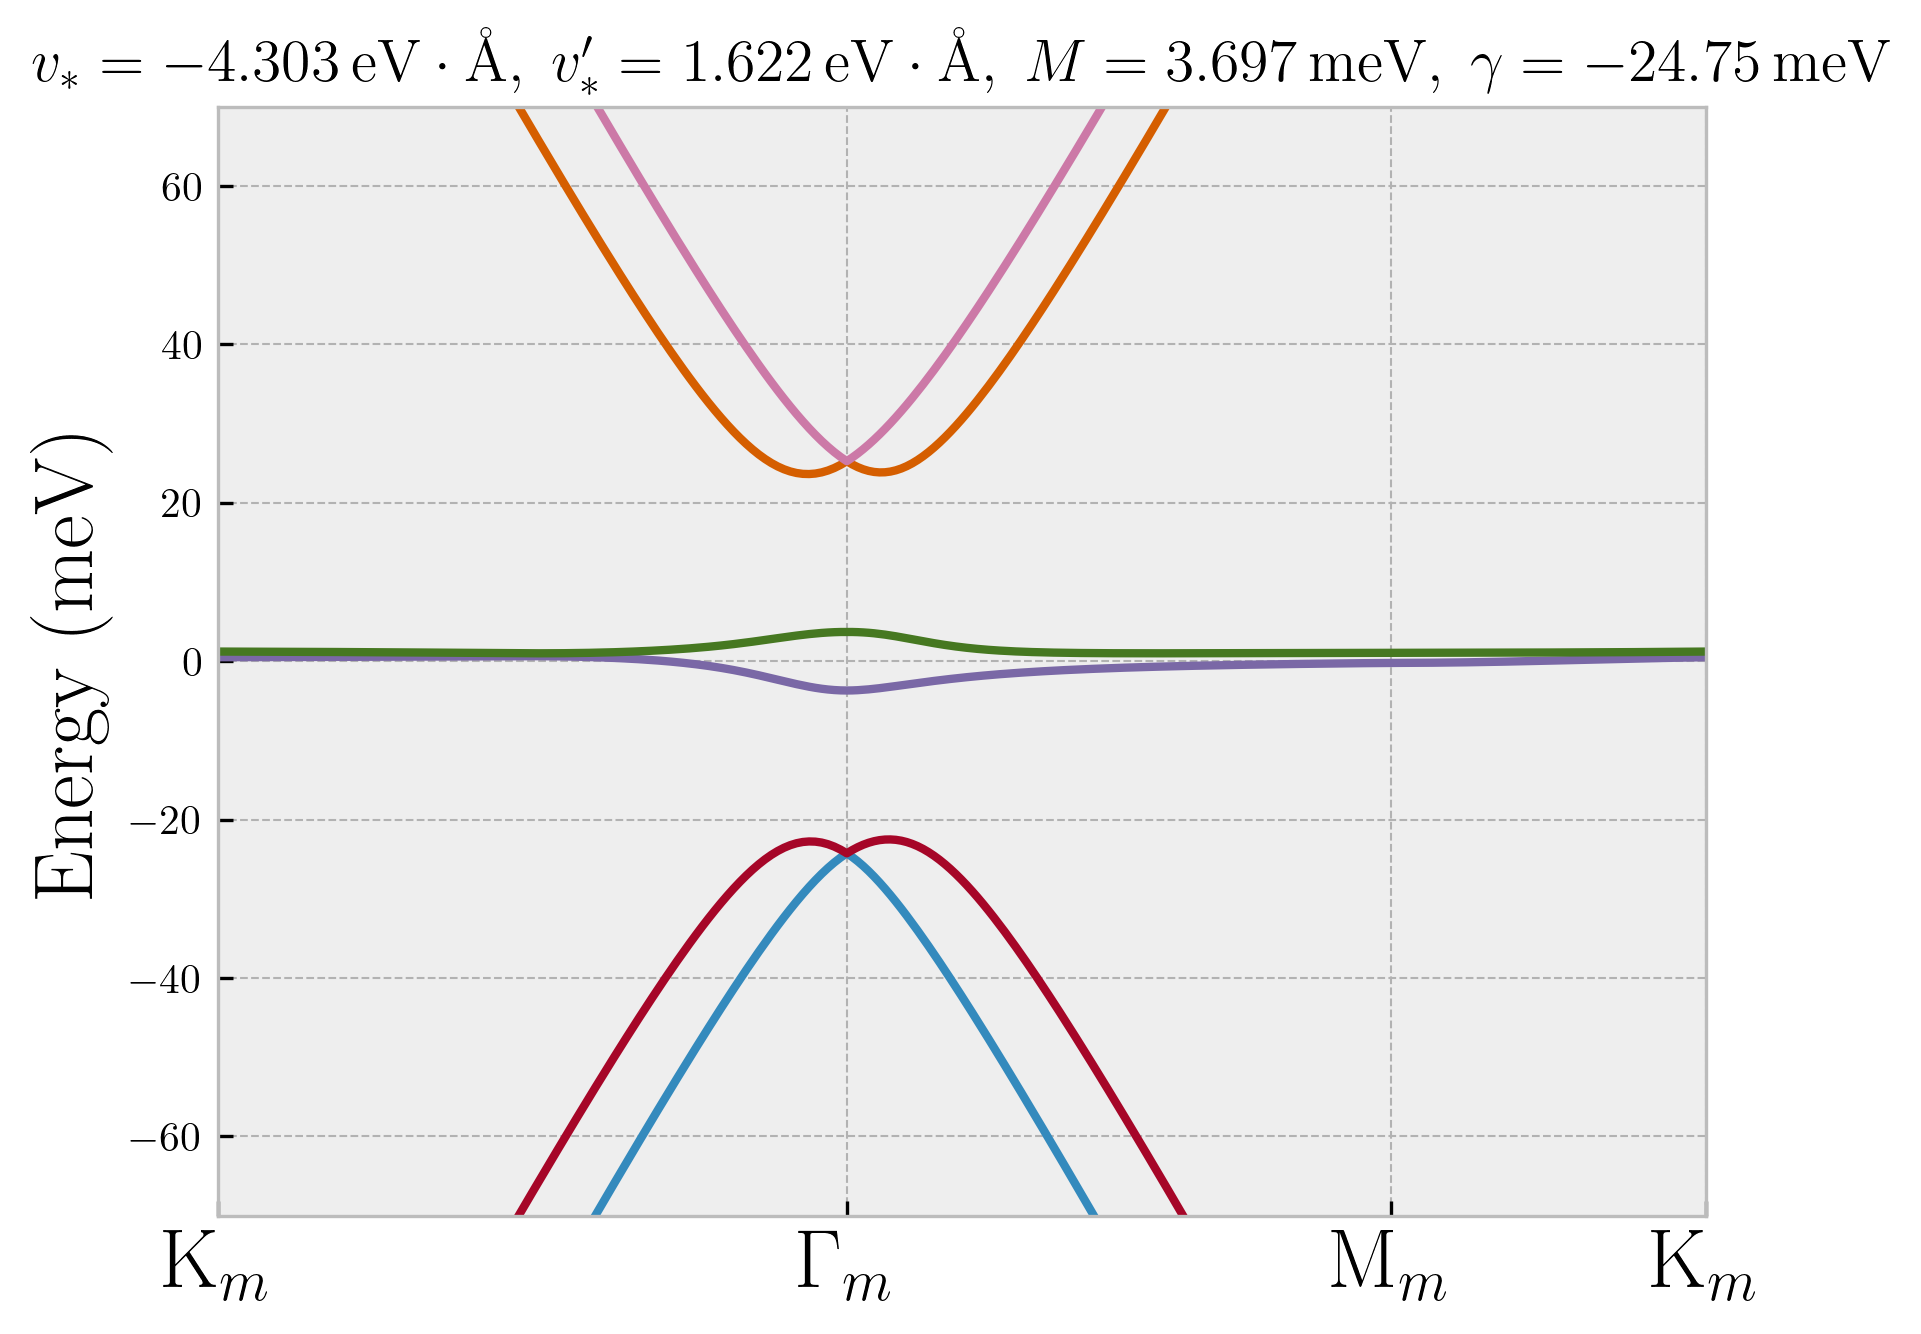
\includegraphics[height=0.35\linewidth]{fig/thf-correct_params.png}
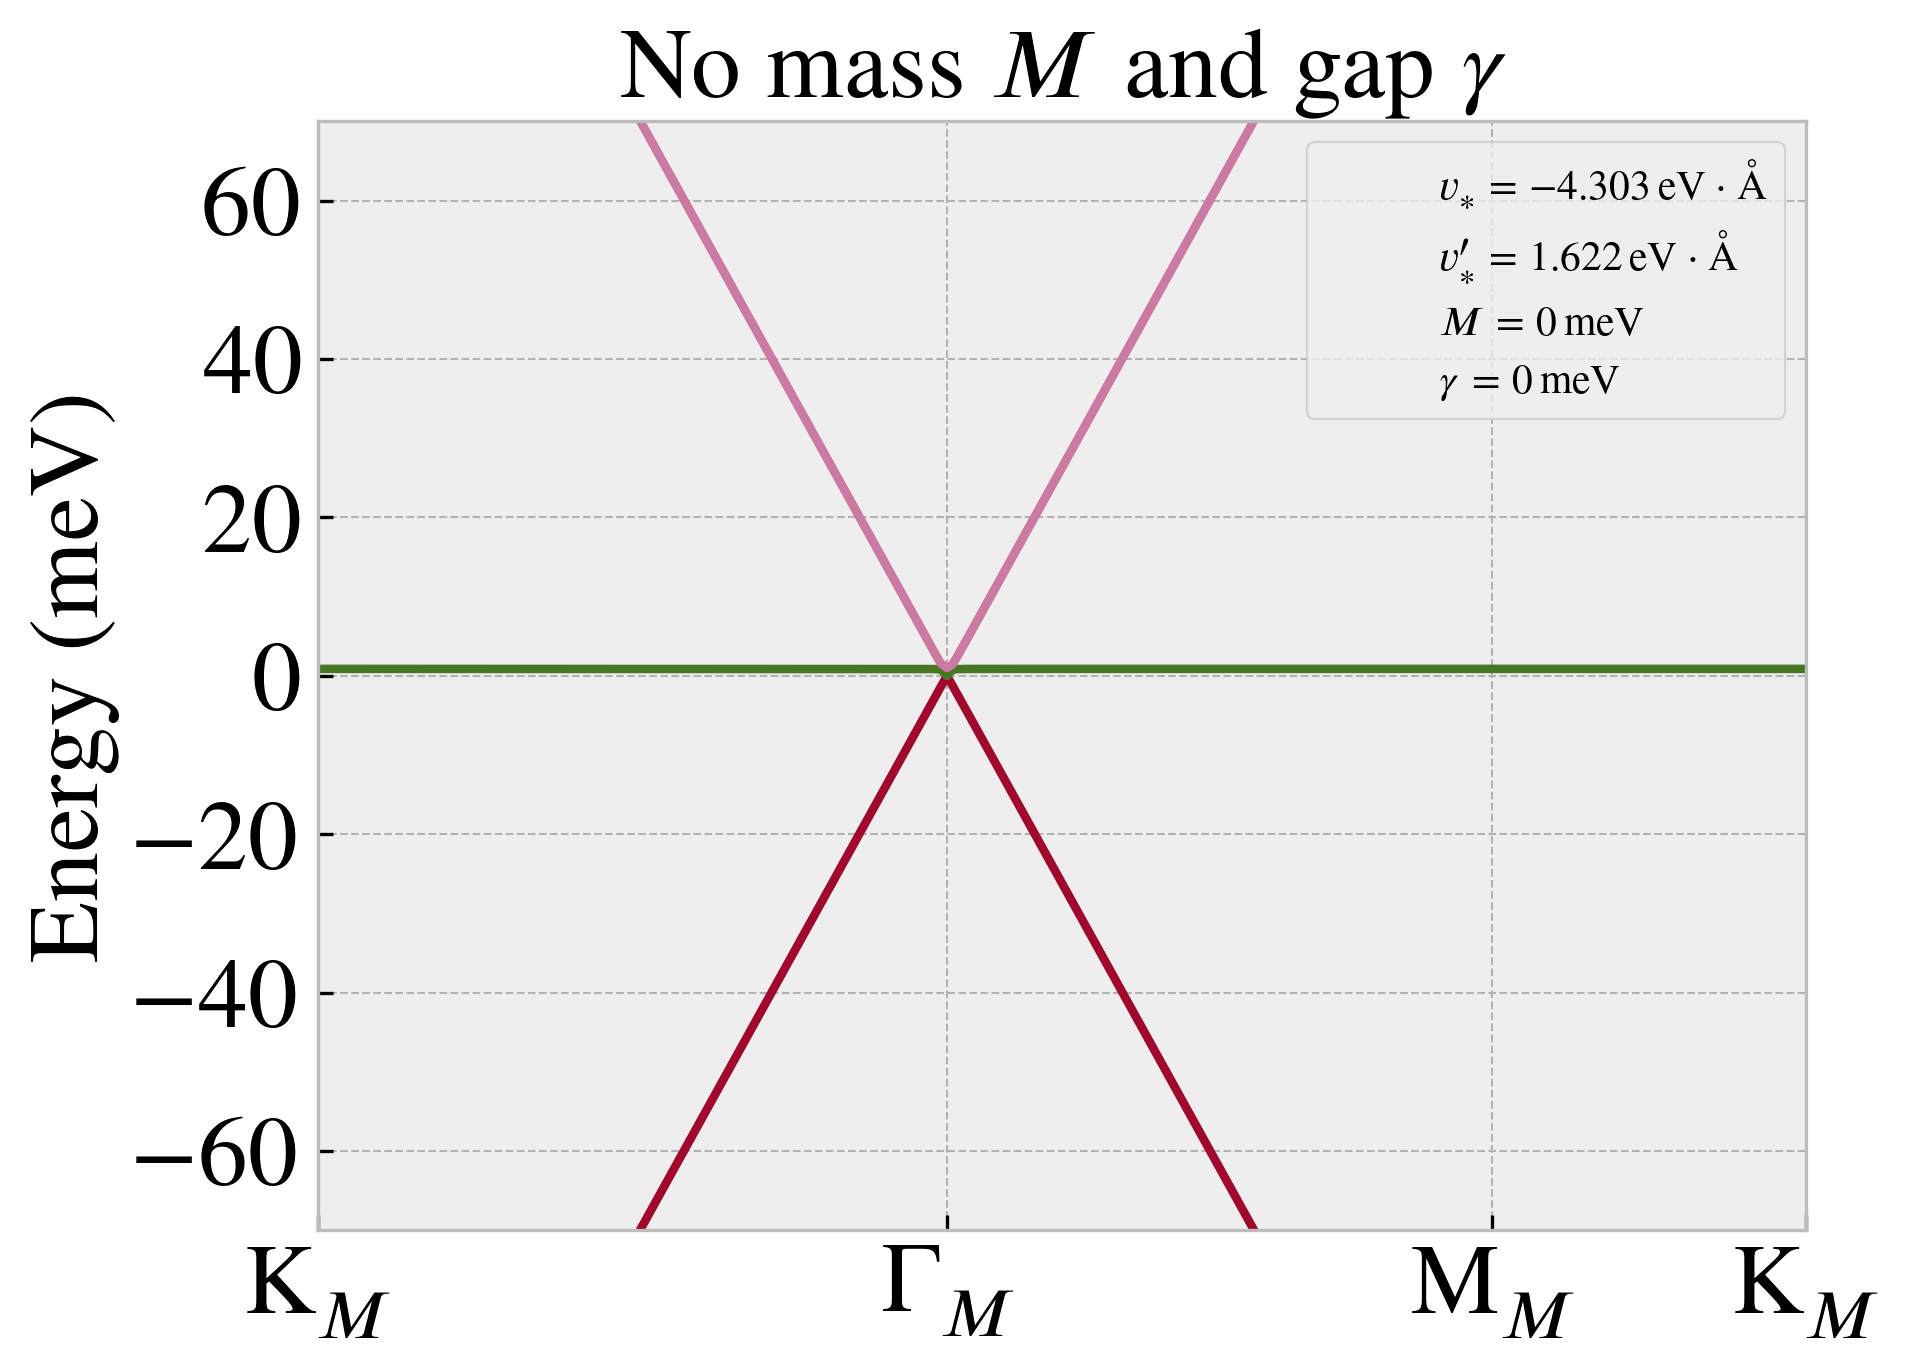
\includegraphics[height=0.35\linewidth]{fig/thf-no_M_no_gamma.png}
%%\caption{}
%\label{fig:thf-correct_params}
%\end{figure}
%\begin{figure}[H]
%\centering
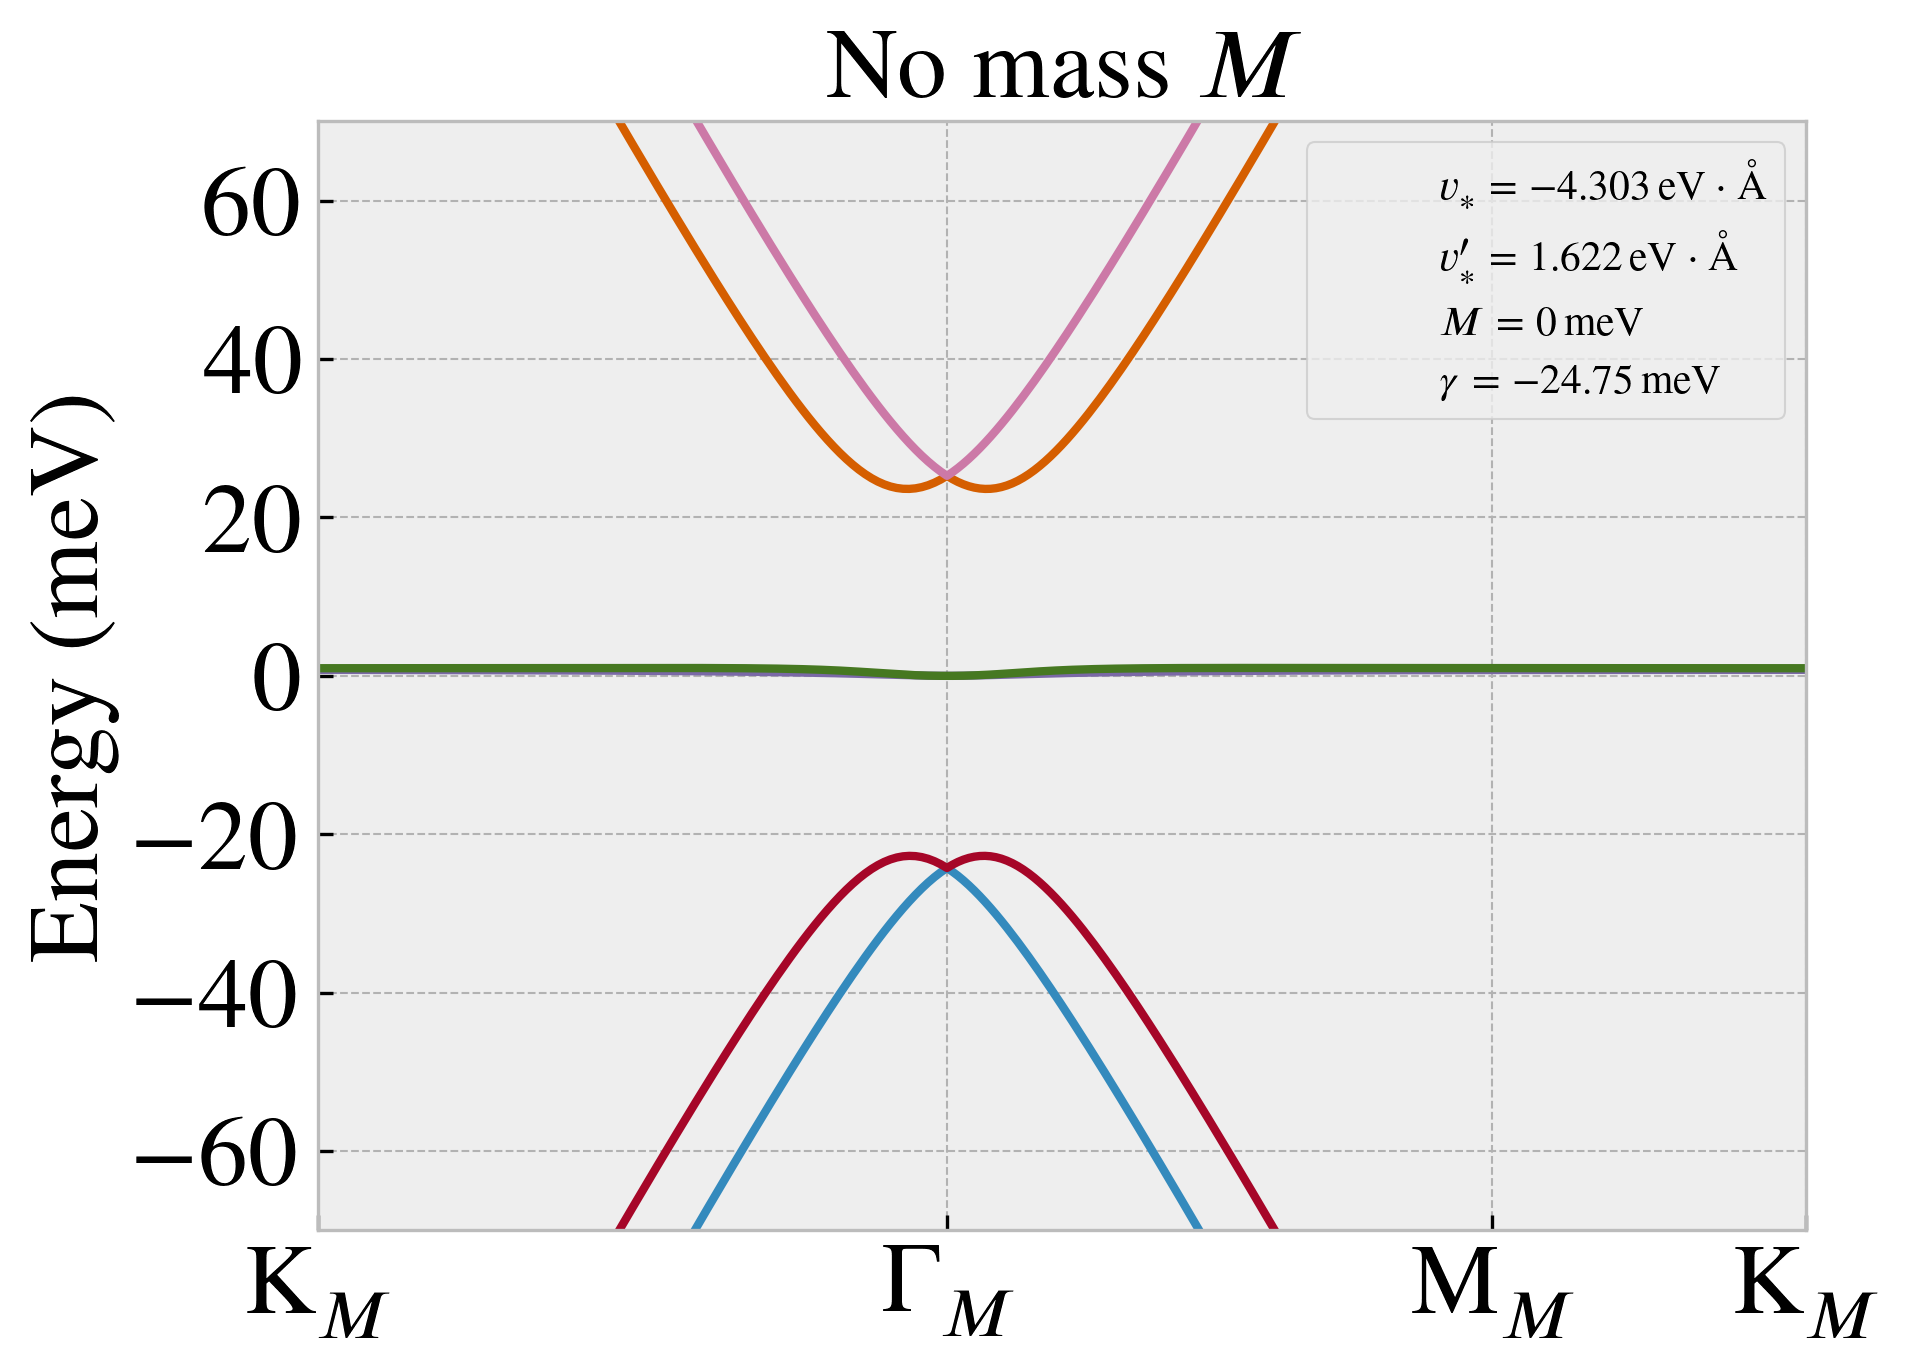
\includegraphics[height=0.35\linewidth]{fig/thf-no_M.png}
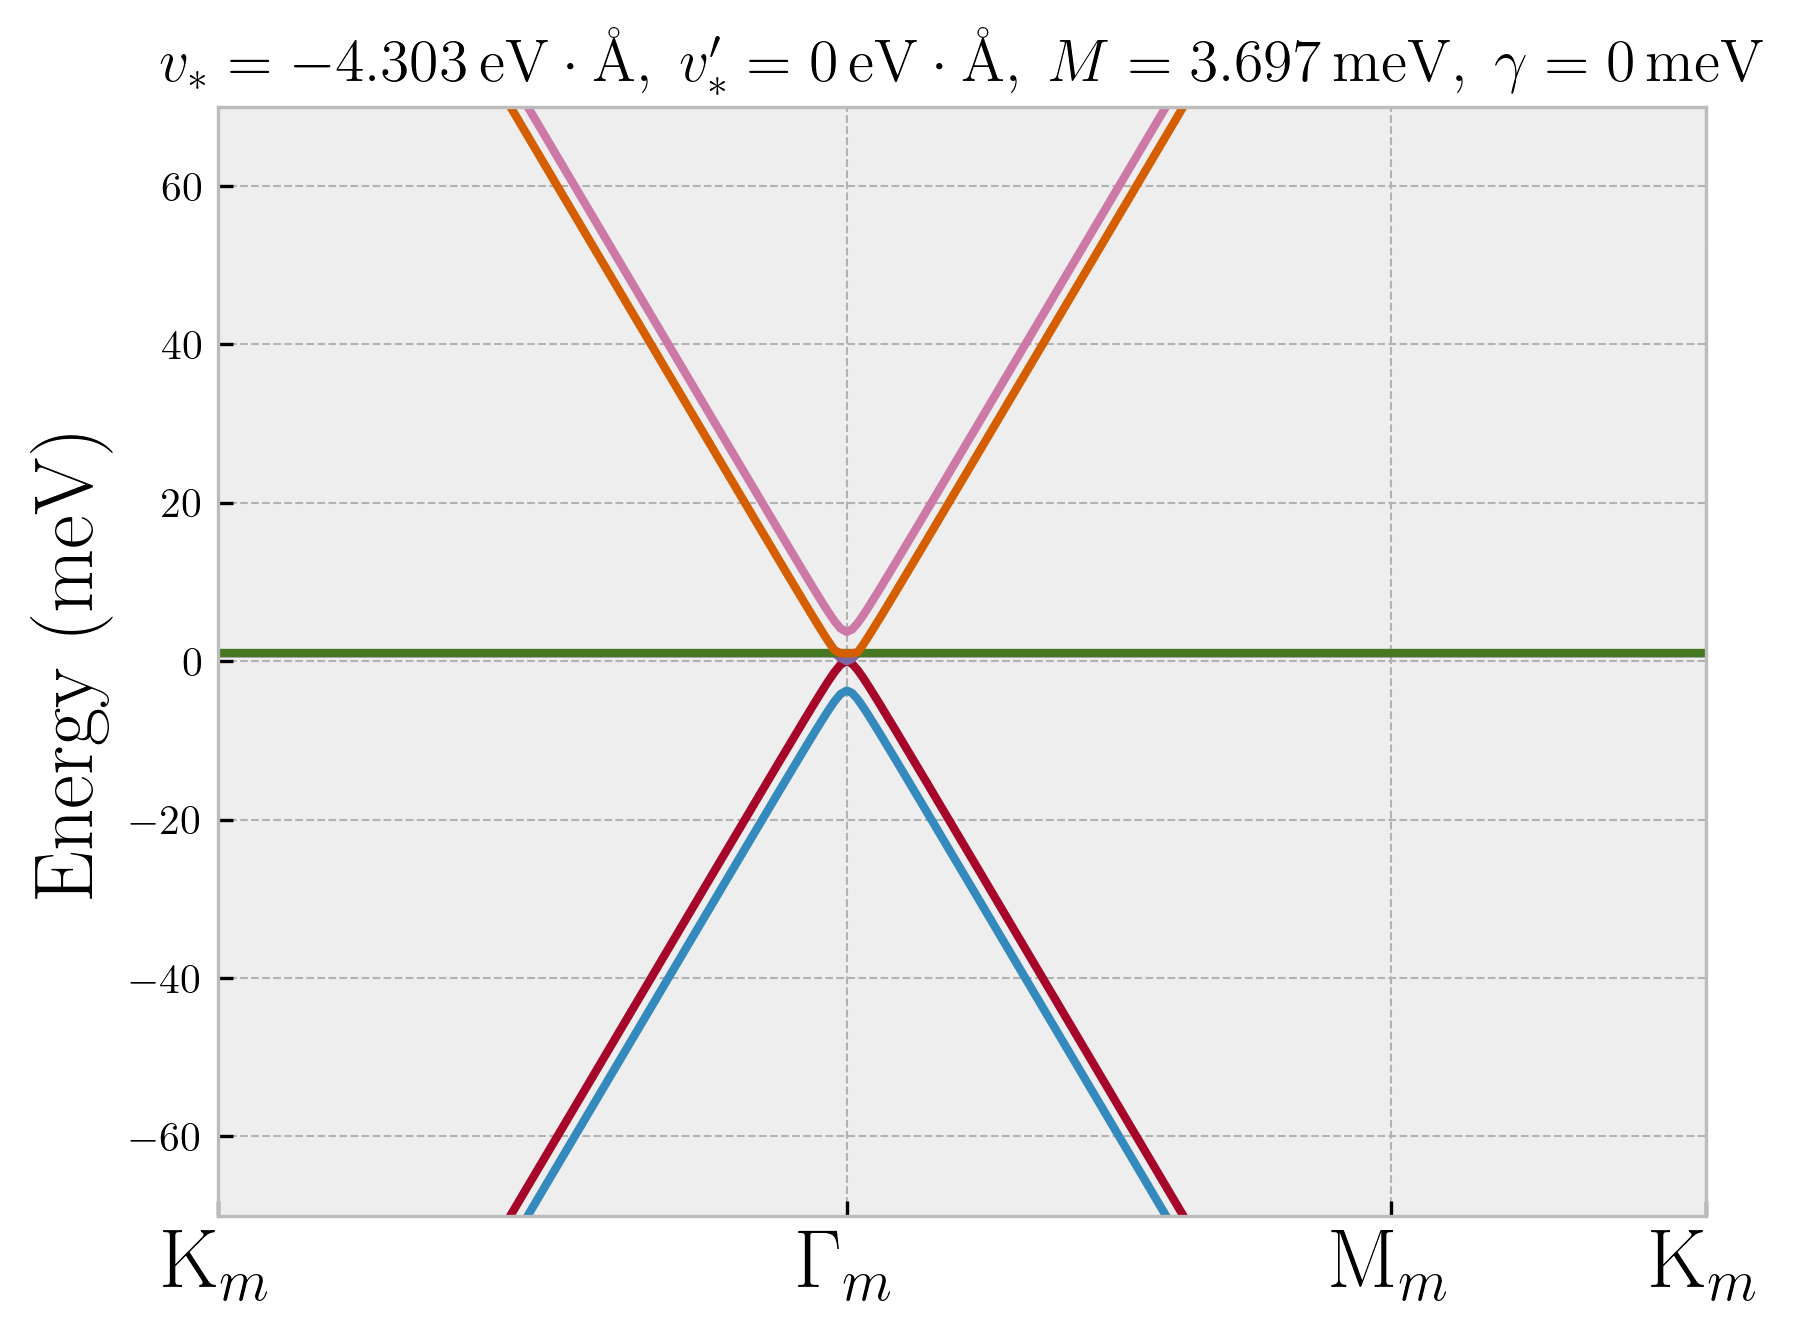
\includegraphics[height=0.35\linewidth]{fig/thf-no_coupling.png}
\caption{Band structures for the 6-band non-interacting Topological Heavy Fermion model, showing the effect of different parameters on the electronic states. Each panel illustrates a variation of the model with certain parameters set to zero.}
\label{fig:thf-exploration}
\end{figure}

%%%%%%%%%%%%%%%%%%%%%%%%%%%%%%%%%%%%%%%%%%%%%%%%%%%%%%%%%%%%%%%%%%%%%%%%%%%%%%%%%%%%%%%%%%%%%%%%%%
\section{Monolayer}
%%%%%%%%%%%%%%%%%%%%%%%%%%%%%%%%%%%%%%%%%%%%%%%%%%%%%%%%%%%%%%%%%%%%%%%%%%%%%%%%%%%%%%%%%%%%%%%%%%

Considering only nearest-neighbors, the hamiltonian of a single unrotated layer of graphene is given by
$$
H_{\text{mono}}(\k) = -t
\begin{pmatrix}
0 & f(\k) \\
f^*(\k) & 0
\end{pmatrix}
, \quad \ell = 1, 2,
$$
where $f = \sum_{i=1}^{3} e^{i \k \vdot \bm{\delta}}$, and $\bm{\delta}$ are the three nearest-neighbor vectors from a site $A$ of the honeycomb lattice.

Expanding in first-order $\k = \K + \q$, where $\K = \frac{4\pi}{3a} (1, 0)$ is the Dirac point of the unrotated layer, we have
$$
H_{\text{mono}}(\K + \q) \approx v_F \, \q \vdot \bm{\sigma}.
$$

%%%%%%%%%%%%%%%%%%%%%%%%%%%%%%%%%%%%%%%%%%%%%%%%%%%%%%%%%%%%%%%%%%%%%%%%%%%%%%%%%%%%%%%%%%%%%%%%%%
\section{BM model review}
%%%%%%%%%%%%%%%%%%%%%%%%%%%%%%%%%%%%%%%%%%%%%%%%%%%%%%%%%%%%%%%%%%%%%%%%%%%%%%%%%%%%%%%%%%%%%%%%%%

The hamiltonian of the BM model is given by
$$
H = H_1 + H_2 + V + V^\dagger,
$$
where $H_1$ and $H_2$ correspond to the layers 1 and 2, and $V$ is the hybridization between them.

\n

For this discussion, we use the reference frame where layer 1 is unrotated and layer 2 is rotated counter-clockwise by an angle $\theta$. Therefore, we have
$$
H_1(\k) = H_{\text{mono}}(\k), \quad H_2(\k) = H_1(R_\theta^{-1}\k),
$$
$$
R_\theta =
\begin{pmatrix}
\cos\theta & -\sin\theta \\
\sin\theta & \cos\theta
\end{pmatrix}.
$$

Also, the Dirac points of each layer are
$$
\K_1 = \K = \frac{4\pi}{3a} (1, 0), \quad \K_2 = R_\theta \K_1 = R_\theta \K,
$$
$$
$$

Therefore, expanding around the Dirac points $\K_1$ and $\K_2$, respectively:
$$
H_1(\K_1 + \q) \approx v_F \, \q \vdot \bm{\sigma}.
$$
$$
\boxed{ H_2(\K_2 + \q) = H_2(R_\theta \K_1 + \q) = H_1(\K_1 + R_\theta^{-1}\q) \approx v_F \, (R_\theta^{-1}\q) \vdot \bm{\sigma} \approx v_F \, (1 - i \theta \sigma_y ) \, \q \vdot \bm{\sigma}. }
$$

If we \textbf{neglect the $\theta$-dependence on $H_2$}, our BM model will be \textbf{particle-hole symmetric}, as defined by Bernevig.

\n

Of course, the more difficult part is due to the hybridization term $V$. It is written on the Bloch basis $\ket{\ell, \alpha, \p}$, where $\ell = 1, 2$ is the layer index, $\alpha = A, B$ is the sublattice index, and $\p$ is the momentum.
We have
$$
V_{\alpha\beta}(\p, \p') = \bra{1, \alpha, \p} H \ket{2, \beta, \p'}.
$$

When we expand both $\p = \K_1 + \q$ and $\p' = \K_2 + \q'$, \textbf{after the BM considerations}, we get
$$
V_{\alpha\beta}(\K + \q, R_\theta \K + \q') \approx
w \sum_{j=1}^{3} \delta_{\q, \q' + \q_j} T_{\alpha\beta}^j,
$$
where $\q_1, \q_2, \q_3$ are the moiré momentum vectors, with absolute value $k_D = 2 \sin(\theta/2) \abs{\K}$. The matrices $T^j_{\alpha\beta}$ are
$$
T_1 = \sigma_0 + \sigma_x
$$
$$
T_2 = \sigma_0 + \cos(\frac{2\pi}{3}) \sigma_x + \sin(\frac{2\pi}{3}) \sigma_y
$$
$$
T_3 = \sigma_0 + \cos(\frac{2\pi}{3}) \sigma_x - \sin(\frac{2\pi}{3}) \sigma_y
$$
\begin{figure}[H]
\centering
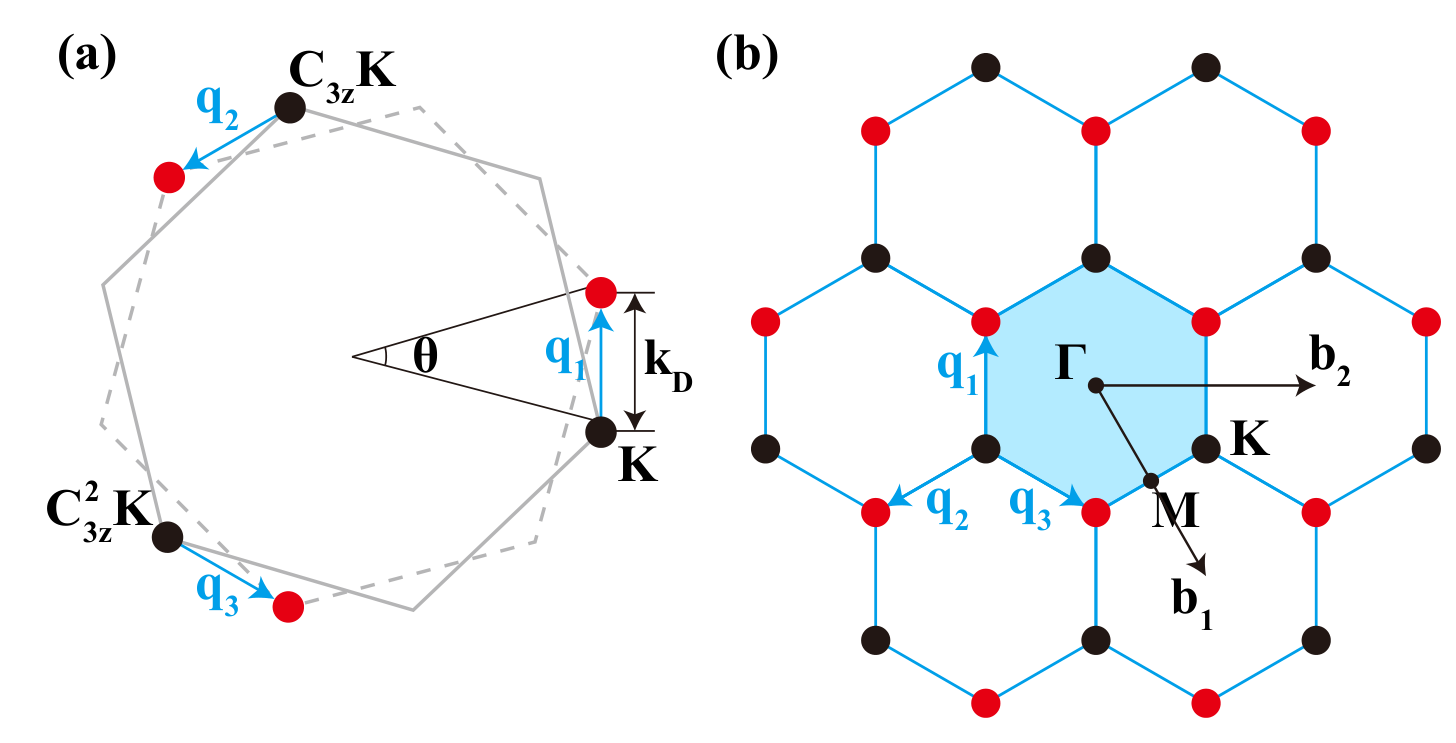
\includegraphics[width=0.8\linewidth]{fig/moire-vectors.png}
\end{figure}

\n

This \textbf{BM model} is called \textbf{MBM-1V (Moiré Band Model - One Valley)} by Bernevig. If we decompose $\q = \k - \Q$, $\q'=\k-\Q'$, where $\Q$ and $\Q'$ belong to the hexagonal lattice formed by adding $\q_{1,2,3}$ iteratively, we can rewrite the hamiltonian as
$$
\boxed{
H_{\Q, \Q'}^{(\text{MBM-1V})}(\k) =
\delta_{\Q,\Q'} v_F (\k-\Q) \vdot \bm{\sigma}
+ w \sum_{j=1}^{3} (\delta_{\Q'-\Q, \q_j} + \delta_{\Q-\Q', \q_j}) T^j.
}
$$

\begin{itemize}
\item This model is \textbf{topological} and is what we have been discussing the whole time.
\item The tables of Bernevig apply to this model, where we consider the Wyckoff position 1a within the THF approach to solve the topological obstruction.
\item Its magnetic space group is $P6'2'2$. Generators: $C_{6z} T$, $C_{2y} T$, $C_{2x}$.
\end{itemize}

\begin{table}[H]
\scriptsize
\caption{Elementary band representations of the magnetic space group $P6'2'2$.}
\centering
\begin{tabular}{|c|c|c|c|c|c|c|c|c|}
\hline
Wyckoff & \multicolumn{3}{c|}{$1a$} & \multicolumn{3}{c|}{$2c$} & \multicolumn{2}{c|}{$3f$} \\
\cline{1-9}
Site sym. & \multicolumn{3}{c|}{$6'2'2$, $32$} & \multicolumn{3}{c|}{$32$, $32$} & \multicolumn{2}{c|}{$2'2'2$, $2$} \\
\cline{1-9}
EBR & $G_{A_1}^{1a}(1)$ & $G_{A_2}^{1a}(1)$ & $G_{E}^{1a}(2)$ & $G_{A_1}^{2c}(2)$ & $G_{A_2}^{2c}(2)$ & $G_{E}^{2c}(4)$   & $G_{A}^{3f}(3)$ & $G_{B}^{3f}(3)$ \\
\hline
$\Gamma$ & $\Gamma_1(1)$ & $\Gamma_2(1)$ & $\Gamma_3(1)$ & $2\Gamma_1(1)$ & $2\Gamma_2(1)$ & $2\Gamma_3(2)$ & $\Gamma_1(1)+\Gamma_3(2)$ & $\Gamma_2(1)+\Gamma_3(2)$ \\
\hline
$K$ & $K_1(1)$ & $K_1(1)$ & $K_2 K_3(2)$ & $K_2 K_3(2)$ & $K_2 K_3(2)$ & $2K_1(1) + K_2 K_3(2)$ & $K_1(1)+K_2 K_3(2)$ & $K_1(1)+K_2 K_3(2)$ \\
\hline
$M$ & $M_1(1)$ & $M_2(1)$ & $M_1(1)+M_2(1)$ & $2M_1(1)$ & $2M_2(1)$ & $2M_1(1)+2M_2(1)$ & $2M_1(1)+M_2(1)$ & $M_1(1)+2M_2(2)$ \\
\hline
\end{tabular}
\label{tab:ebr-P6'2'2}
\end{table}

\begin{table}[H]
\caption{Character table of irreps at high symmetry momenta in magnetic space group $P6'2'2$.}
\centering
\begin{tabular} { c c c c | c c c | c c c }
\cline{1-10}
$\P$ & $\P \Gamma_1$ & $\P \Gamma_2$ & $\P \Gamma_3$ & $\P$ & $\P M_1$ & $\P M_2$ & $\P$ & $\P K_1$ & $\P K_2K_3$ \\
\cline{1-10}
$E$ & $\P1$ & $\P1$ & $\P2$ & $\P E$ & $\P1$ & $\P1$ & $\P E$ & $\P1$ & $\P2$ \\
$2 C_3$ & $\P1$ & $\P1$ & $ -1$ & $\P C_2'$ & $\P1$ & $ -1$ & $\P C_3$ & $\P1$ & $ -1$ \\
$3 C_2'$ & $\P1$ & $ -1$ & $\P0$ & $\P$ & $\P$ & $\P$ & $\P C_3^{-1}$ & $\P1$ & $-1$ \\
\cline{1-10}
\end{tabular}
\label{tab:char-P6'2'2}
\end{table}

%%%%%%%%%%%%%%%%%%%%%%%%%%%%%%%%%%%%%%%%%%%%%%%%%%%%%%%%%%%%%%%%%%%%%%%%%%%%%%%%%%%%%%%%%%%%%%%%%%
\section{There exists another model}
%%%%%%%%%%%%%%%%%%%%%%%%%%%%%%%%%%%%%%%%%%%%%%%%%%%%%%%%%%%%%%%%%%%%%%%%%%%%%%%%%%%%%%%%%%%%%%%%%%

According to Bernevig: ``The MBM-1V is half of the TBG system, with similar physics taking place in the electron states around $\K'$''. A model with the two valleys can be written as
$$
\boxed{
H_{\Q, \Q'}^{(\text{MBM-2V})}(\k) =
\delta_{\Q,\Q'} v_F (\k-\Q) \vdot \bm{\sigma} \otimes \tau_z
+ w \sum_{j=1}^{3} (\delta_{\Q'-\Q, \q_j} + \delta_{\Q-\Q', \q_j}) T^j \otimes \tau_0.
}
$$

Here $\tau_z$ and $\tau_0$ are the Pauli and identity matrix representing the valley degree of freedom.

\begin{itemize}
\item This model is \textbf{apparently different} from the latter, and \textbf{is not topological}. You can decompose it in EBR's as $G_{A_1}^{2c} + G_{A_2}^{2c}$.
\item The tables of Rennella apply to this model. There the authors (Vafek, Rennella, Angeli, Koshino, etc) consider Wyckoff position 2c, because these positions really correspond to symmetry-adapted exponentially localized Wannier functions.
\item The magnetic space group is $P6221'$. Generators: $C_{6z}$, $C_{2y}$, $C_{2x}$, $T$.
\end{itemize}

\begin{table}[H]
\caption{Elementary band representations generated from Wyckoff position $2c$ of the space group $P622$.}
\centering
\begin{tabular}{|c|c|c|c|}
\hline
Wyckoff & \multicolumn{3}{c|}{$2c$} \\
\cline{1-4}
Site sym. & \multicolumn{3}{c|}{$32$} \\
\cline{1-4}
EBR & $G_{A_1}^{2c}(2)$ & $G_{A_2}^{2c}(2)$ & $G_{E}^{2c}(4)$  \\
\hline
$\Gamma$ & $\Gamma_1(1) + \Gamma_4(1)$ & $\Gamma_2(1) + \Gamma_3(1)$ & $\Gamma_5(2) + \Gamma_6(2)$ \\
\hline
$K$ & $K_3(2)$ & $K_3(2)$ & $K_1(1) + K_2(1) + K_3(2)$ \\
\hline
$M$ & $M_1(1) + M_4(1)$ & $M_2(1) + M_3(1)$ & $M_1(1) + M_2(1) + M_3(1) + M_4(1)$ \\
\hline
\end{tabular}
\label{tab:ebr-P622}
\end{table}

\begin{table}[H]
\caption{Character table of irreps at high symmetry momenta in space group $P622$.}
\scriptsize
\centering
\begin{tabular} { c c c c c c c | c c c c c | c c c c }
\cline{1-16}
$\P$ & $\P \Gamma_1$ & $\P \Gamma_2$ & $\P \Gamma_3$ & $\P \Gamma_4$ & $\P \Gamma_5$ & $\P \Gamma_6$ & $\P$ & $\P M_1$ & $\P M_2$ & $\P M_3$ & $\P M_4$ & $\P$ & $\P K_1$ & $\P K_2$ & $\P K_3$\\
\cline{1-16}
$E$      & $\P1$ & $\P1$ & $\P1$ & $\P1$ & $\P2$ & $\P2$ & $E$     & $\P1$ & $\P1$  & $\P1$ & $\P1$ & $E$      & $\P1$ & $\P1$ & $\P2$ \\
$2C_6$   & $\P1$ & $\P1$ & $ -1$ & $ -1$ & $ -1$ & $\P1$ & $C_2$   & $\P1$ & $\P1$  & $ -1$ & $ -1$ & $C_3$    & $\P1$ & $\P1$ & $ -1$ \\
$2C_3$   & $\P1$ & $\P1$ & $\P1$ & $\P1$ & $ -1$ & $ -1$ & $C_2'$  & $\P1$ & $ -1$  & $ -1$ & $\P1$ & $3C_2''$ & $\P1$ & $ -1$ & $\P0$ \\
$C_2$    & $\P1$ & $\P1$ & $ -1$ & $ -1$ & $\P2$ & $ -2$ & $C_2''$ & $\P1$ & $ -1$  & $\P1$ & $ -1$ &          &       &       &       \\
$3C_2'$  & $\P1$ & $ -1$ & $ -1$ & $\P1$ & $\P0$ & $\P0$ &         &       &        &       &       &          &       &       &       \\
$3C_2''$ & $\P1$ & $ -1$ & $\P1$ & $ -1$ & $\P0$ & $\P0$ &         &       &        &       &       &          &       &       &       \\
\cline{1-16}
\end{tabular}
\label{tab:char-P622}
\end{table}

Compare tables \ref{tab:ebr-P622} and \ref{tab:char-P622} with tables 2.5 and (2.1, 2.3) of Rennella \cite{thesis_rennella}, respectively.




%%%%%%%%%%%%%%%%%%%%%%%%%%%%%%%%%%%%%%%%%%%%%%%%%%%%%%%%%%%%%%%%%%%%%%%%%%%%%%%%%%%%%%%%%%%%%%%%%%
%%%%%%%%%%%%%%%%%%%%%%%%%%%%%%%%%%%%%%%%%%%%%%%%%%%%%%%%%%%%%%%%%%%%%%%%%%%%%%%%%%%%%%%%%%%%%%%%%%


%%%%%%%%%%%%%%%%%%%%%%%%%%%%%%%% COMMENT THIS TO COMPILE main.tex %%%%%%%%%%%%%%%%%%%%%%%%%%%%%%%%
%%%-----
%%% Referências bibliográficas
%%%-----
%\addcontentsline{toc}{chapter}{\bibname}
%%\bibliographystyle{abntex2-num}
%\bibliography{citations}
%\bibliographystyle{ieeetr}
%\end{document}
%%%%%%%%%%%%%%%%%%%%%%%%%%%%%%%% COMMENT THIS TO COMPILE main.tex %%%%%%%%%%%%%%%%%%%%%%%%%%%%%%%%
